\subsection{Komponenten}
\label{ss:komponenten}
Nachfolgend werden alle physischen Elemente beschrieben und vereinzelt mit Bildern veranschaulicht. Die Abbildung \ref{fig:blockdiagramm} zeigt eine Übersicht aller Komponenten.

\begin{figure}[h!]
	\centering
	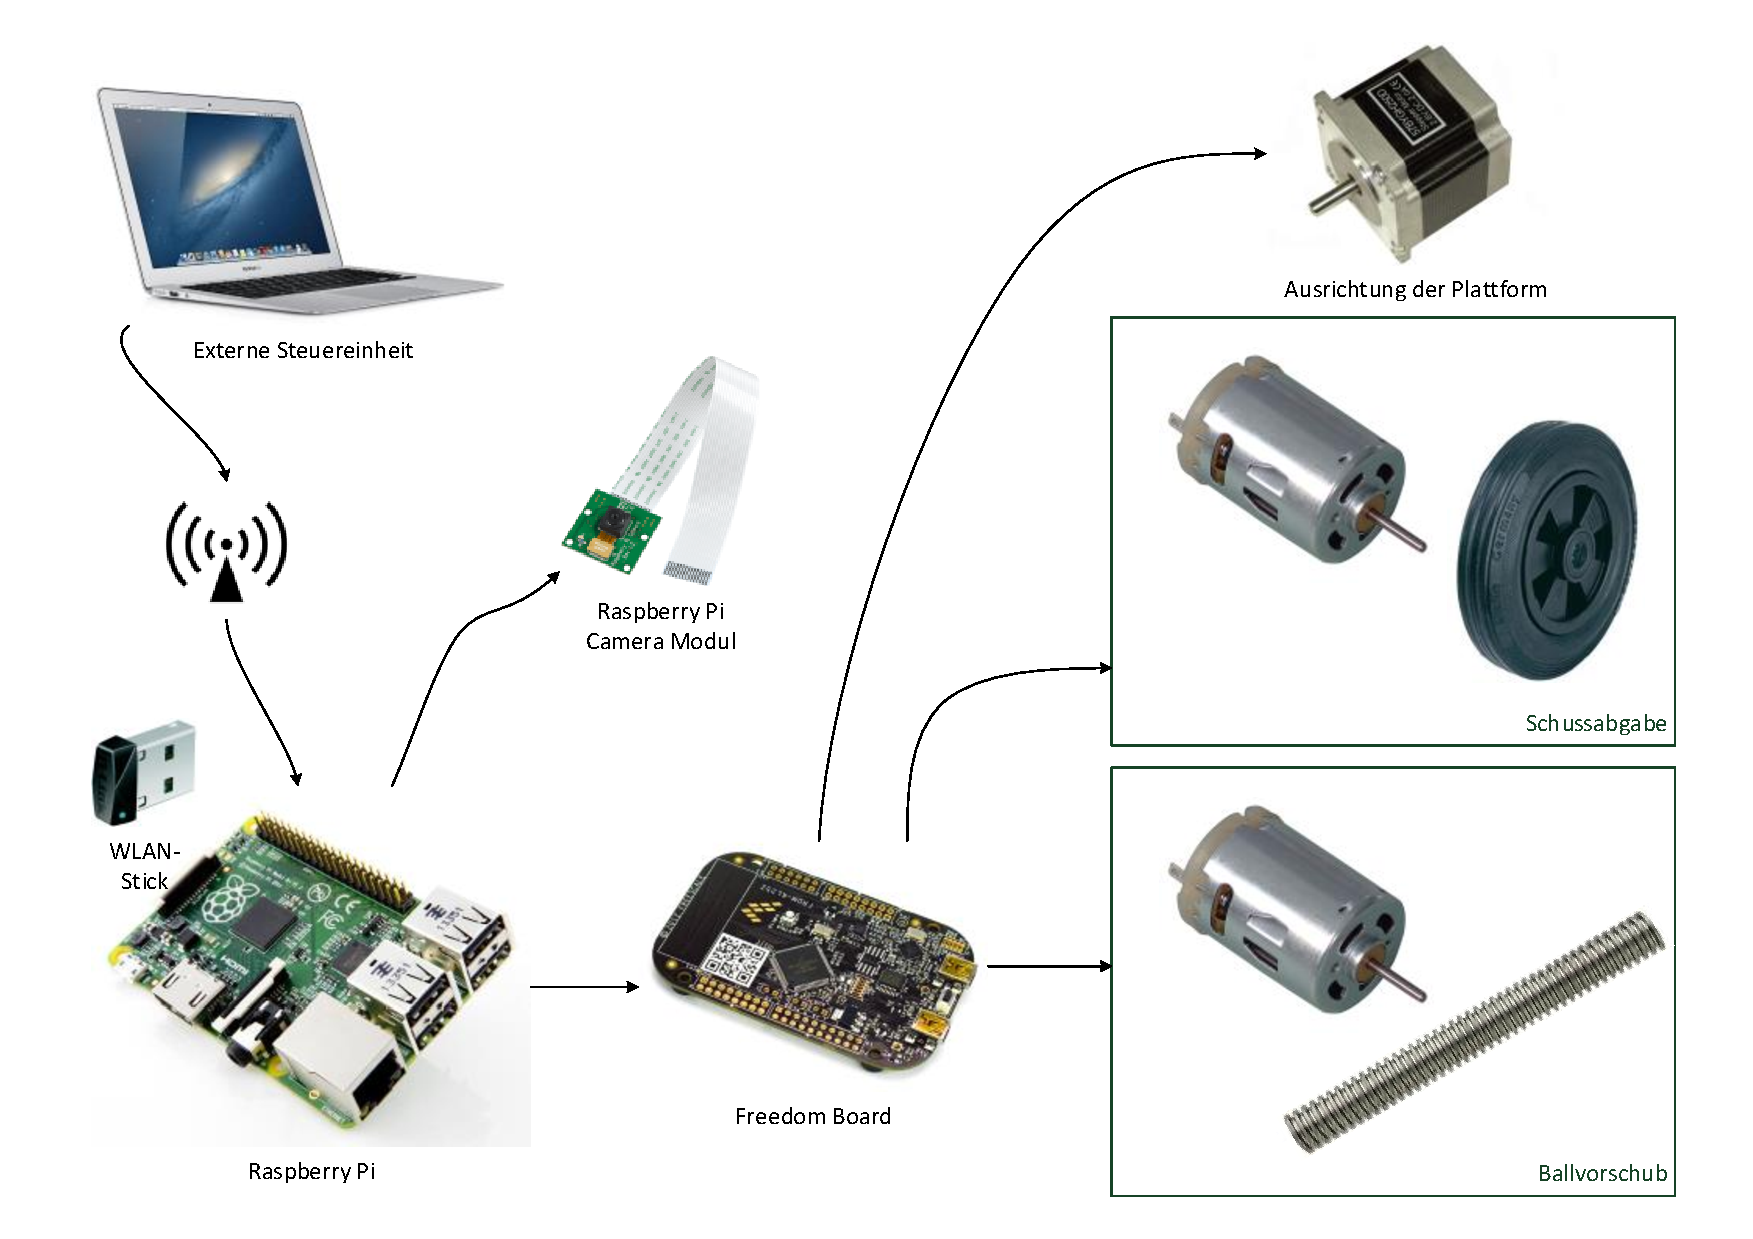
\includegraphics[width=0.9\linewidth]{../../fig/blockdiagramm}
	\caption{Blockdiagramm}
	\label{fig:blockdiagramm}
\end{figure}

\subsubsection{Drehrad}
Das Drehrad ist für die Beschleunigung des Balles zuständig. Durch die Rotation des Rades wird der Tennisball auf die geforderte Geschwindigkeit gebracht. Die erreichte Flugweite hängt zu einem sehr grossen Teil von der Genauigkeit des Drehrades ab. Zudem muss das Drehrad imstande sein, geringe Durchmesseränderungen des Tennisballes auszugleichen. Dazu stehen zwei Lösungsansätze zur Verfügung. Bei der ersten Variante ist die Achse seitlich im Gestell mit Zugfedern befestigt und das Drehrad besteht aus einem harten Material. Die Zugfedern sorgen für einen konstanten Anpressdruck auf den Ball. Diese Variante mit der beweglichen Achse hat den Nachteil, dass der Riemenspanner für den Zahnriemen anspruchsvoller wird. Bei der zweiten Variante ist die Achse fix mit dem Gestell verbunden. Um einen konstanten Anpressdruck auf den Ball zu garantieren, muss die Oberfläche des Drehrades elastisch sein. Dies kann beispielsweise mit einem weichen Gummi- Modellbaurad erreicht werden. Eine weitere Möglichkeit besteht darin, ein Rad mit einer weichen Oberfläche zu versehen. Zum Beispiel mit einer Gummimatte oder Dämmmaterial (Akustisch). Zum jetzigen Zeitpunkt wird die zweite Variante bevorzugt. Die Achse ist bei beiden Varianten seitlich im Gestell gelagert.

\subsubsection{Basisaufbau}
Damit wir unsere Zielvorgabe von unter zwei Kilogramm erreichen können, wird das Gestell aus Holz oder eventuell aus Plexiglas hergestellt. Diese Variante hat den Vorteil, dass das Gehäuse auf der Laserschneidemaschine hergestellt werden kann. Holz oder Plexiglas hat jedoch den Nachteil, dass eventuelle Anbauten wie die Lagerung für das Drehrad in separaten Metallbuchsen erfolgen müssen. Das Gestell besteht aus vier Hauptelementen. Der Grundplatte, der Platte für den Aufbau und die beiden seitlichen Elemente des Aufbaus.

\subsubsection{Freedomboard}
% to do


\subsubsection{Raspberry Pi}
% to do


\subsubsection{Kamera}
\label{subsub:kamera}
% to do


\subsubsection{Externe Steuerungseinheit}
Die externe Steuerungseinheit (bzw. das Bedienelement) dient dazu um den ganzen Prozess mittels eines Start-Signals zu starten. Zum Ende des Prozesses erhält es das Stopp-Signal. Diese Kommunikationspfade müssen gemäss Anforderungen drahtlos erfolgen. \\
Ein weiterer wichtiger Punkt ist die Kalibrierung der Funktion "Ortung des Korbes". In der Umsetzung wird eine Benutzeroberfläche erstellt, welche auf der externen Steuerungseinheit betrieben wird (siehe UI-Skizze in Abschnitt \ref{ss-config-paramater-ortung-orb}).\\
Ein Notebook kann all diese Anforderungen problemlos umsetzen. Heutzutage ist das auch auf einem Smartphone oder Tablet kein Problem mehr. Es wird jedoch das Notebook aus folgenden Gründen bevorzugt:

\begin{itemize}
	\item Plattformunabhängigkeit: Die Implementation für das Notebook erfolgt in Java. Für jedes gängige Betriebssystem gibt eines JVM (Java Virtual Machine).
	\item Know-How: In der Java-Entwicklung ist ein breites Know-How innerhalb des Teams vorhanden.
	\item Bewährt: Java ist einer der meist genutzten Programmiersprachen und hat sich bewährt.
\end{itemize}

Es wird eine Rich-Client Implementation gewählt, weil dann sofort eine Plattform zur Verfügung steht, falls ressourcenintensive Berechnungen während des Prozess durchgeführt werden müssen. Gemäss Tests und Versuchen sollte dies jedoch nicht der Fall ein.





\subsubsection{Antriebe}
% to do


\subsubsection{Netzteile}
% to do

